% Hybrid Quantum-Classical Knowledge Graph Drug Repurposing — A0 portrait poster
%
% Compile:
%   cd docs/poster
%   pdflatex poster && pdflatex poster
%
% Or use the helper:
%   bash scripts/build_poster.sh
%
% Format: A0 portrait, tikzposter (no external poster theme files required).

\documentclass[25pt, a0paper, portrait, margin=0mm,
               innermargin=15mm, blockverticalspace=10mm,
               colspace=10mm, subcolspace=8mm]{tikzposter}

\usepackage{lmodern}
\usepackage[T1]{fontenc}
\usepackage[utf8]{inputenc}
\usepackage{amsmath, amssymb}
\usepackage{graphicx}
\usepackage{booktabs}
\usepackage{xcolor}
\usepackage{hyperref}
\usepackage{tcolorbox}
\usetikzlibrary{positioning, arrows.meta, shapes}

\hypersetup{colorlinks=true, urlcolor=blue!60!black, linkcolor=black, citecolor=blue!50!black}

% --- Theme: clean academic look (white background, subtle accents) ----------
\definecolor{qggblue}{RGB}{20, 70, 140}
\definecolor{qgglight}{RGB}{220, 230, 250}
\definecolor{qggaccent}{RGB}{200, 60, 60}
\definecolor{qggsoft}{RGB}{245, 247, 252}

\usetheme{Default}
\usecolorstyle{Russia}
\colorlet{titlebgcolor}{qggblue}
\colorlet{titlefgcolor}{white}
\colorlet{blocktitlebgcolor}{qggblue}
\colorlet{blocktitlefgcolor}{white}
\colorlet{blockbodybgcolor}{white}
\colorlet{blockbodyfgcolor}{black}
\colorlet{backgroundcolor}{qggsoft}
\colorlet{framecolor}{qggblue}

\usebackgroundstyle{Empty}
\usetitlestyle{Default}
\useblockstyle{Default}

% --- Title block ------------------------------------------------------------
\title{Hybrid Quantum-Classical Knowledge Graph for Drug Repurposing Across Hetionet}
\author{J.~Beale$^{1\ast}$ \quad M.~Jack$^1$ \quad R.~Robinson$^1$ \quad N.~Elsayed$^1$}
\institute{$^1$Quantum Global Group \quad\quad $^\ast$\texttt{beale@quantumglobalgroup.com}}

\begin{document}

\maketitle

% ============================================================================
% ROW 1 — three columns: Motivation | Architecture | Headline result
% ============================================================================

\begin{columns}

% --- Motivation -------------------------------------------------------------
\column{0.33}
\block{1.~Motivation}{
\textbf{The repurposing gap.}
Bringing a new drug to market costs \$2.6B and takes 10--15 years.
Repurposing a known drug to a new disease cuts that to 3--5 years
at a fraction of the cost --- but the search space is vast
($\sim$10{,}000 approved compounds $\times$ $\sim$10{,}000 indications).

\vspace{4mm}
\textbf{Why hybrid quantum--classical?}
Knowledge-graph (KG) embeddings capture relational structure across
biomedical entities; quantum kernels encode that structure in a
high-dimensional Hilbert space without explicit feature engineering.
A stacking ensemble lets the two views vote.

\vspace{4mm}
\textbf{Beyond benchmarks.}
We add single-cell disease signatures and drug perturbation
reversal scores so candidates are biologically grounded ---
not just topologically plausible.
}

% --- Architecture diagram --------------------------------------------------
\column{0.33}
\block{2.~Pipeline architecture}{
\begin{center}
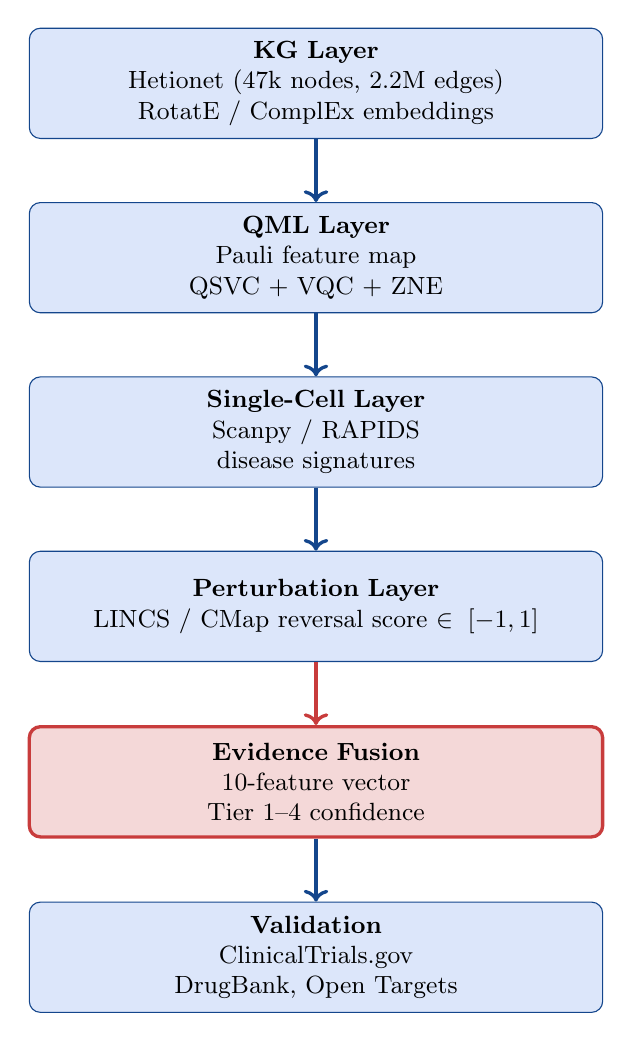
\begin{tikzpicture}[node distance=8mm, font=\small,
    every node/.style={align=center, rounded corners=4pt, minimum height=14mm,
                       inner sep=4pt}]
  \node[fill=qgglight, draw=qggblue, text width=70mm] (kg)
        {\textbf{KG Layer}\\Hetionet (47k nodes, 2.2M edges)\\RotatE / ComplEx embeddings};
  \node[fill=qgglight, draw=qggblue, text width=70mm, below=of kg] (qml)
        {\textbf{QML Layer}\\Pauli feature map\\QSVC + VQC + ZNE};
  \node[fill=qgglight, draw=qggblue, text width=70mm, below=of qml] (sc)
        {\textbf{Single-Cell Layer}\\Scanpy / RAPIDS\\disease signatures};
  \node[fill=qgglight, draw=qggblue, text width=70mm, below=of sc] (pert)
        {\textbf{Perturbation Layer}\\LINCS / CMap reversal score $\in [-1, 1]$};
  \node[fill=qggaccent!20, draw=qggaccent, very thick, text width=70mm, below=of pert] (ev)
        {\textbf{Evidence Fusion}\\10-feature vector\\Tier 1--4 confidence};
  \node[fill=qgglight, draw=qggblue, text width=70mm, below=of ev] (val)
        {\textbf{Validation}\\ClinicalTrials.gov\\DrugBank, Open Targets};

  \draw[->, very thick, qggblue] (kg) -- (qml);
  \draw[->, very thick, qggblue] (qml) -- (sc);
  \draw[->, very thick, qggblue] (sc) -- (pert);
  \draw[->, very thick, qggaccent] (pert) -- (ev);
  \draw[->, very thick, qggblue] (ev) -- (val);
\end{tikzpicture}
\end{center}

All layers ship as importable Python packages with a single end-to-end
orchestrator: \texttt{run\_full\_repurposing\_pipeline.py --mode \{kg-only,kg+omics\}}.
}

% --- Headline result -------------------------------------------------------
\column{0.34}
\block{3.~Headline result}{
\begin{tcolorbox}[colback=qgglight, colframe=qggblue, sharp corners,
                  boxrule=2pt, left=4mm, right=4mm, top=3mm, bottom=3mm]
\begin{center}
{\Huge\bfseries PR-AUC = 0.7987}\\[2mm]
\textit{Hetionet Compound-treats-Disease (CtD) sealed test set}
\end{center}
\end{tcolorbox}

\vspace{6mm}
\textbf{Configuration} (preregistered on OSF):
\begin{itemize}
  \item Pauli feature map (5 qubits, reps=2)
  \item RotatE 32d $\to$ PCA $\to$ 5d
  \item Hard degree-corrupt negatives
  \item Stacking ensemble (QSVC + RF + LR)
  \item Linear + Richardson zero-noise extrapolation
\end{itemize}

\vspace{4mm}
\textbf{Reproducibility}: paired bootstrap CI ($n=$1000),
sealed test set wrapper, deterministic seeds, GitHub Actions CI gate.
}

\end{columns}

% ============================================================================
% ROW 2 — two columns: Methods | Per-disease results
% ============================================================================

\begin{columns}

% --- Methods ---------------------------------------------------------------
\column{0.5}
\block{4.~Methods}{
\textbf{Knowledge graph.} Hetionet v1.0 — 47{,}031 nodes across 11 types
(Compound, Disease, Gene, Pathway, Anatomy, $\ldots$) and 2{,}250{,}197
typed edges. Compound-treats-Disease (CtD) selected as the binary
prediction task.

\vspace{3mm}
\textbf{Quantum feature map.} Each compound-disease pair is encoded as
\[
|\phi(x)\rangle = U_{\Phi(x)} H^{\otimes n} |0\rangle^{\otimes n}, \qquad
U_{\Phi(x)} = \text{PauliFeatureMap}(x)
\]
on $n=5$ qubits, reps$=2$. Quantum kernel
$K(x_i, x_j) = |\langle\phi(x_i)|\phi(x_j)\rangle|^2$ feeds a
classical SVC (QSVC).

\vspace{3mm}
\textbf{Disease signatures.} Single-cell RNA-seq per condition
$\to$ Wilcoxon DE $\to$ up/down gene lists per cell type.
Consensus signature filters genes appearing in $\geq 2$ cell types.

\vspace{3mm}
\textbf{Reversal score.}
\[
R(d, c) = \frac{|U_d \cap D_c| + |D_d \cap U_c| - |U_d \cap U_c| - |D_d \cap D_c|}{(|U_d \cup D_d| + |U_c \cup D_c|)/2}
\in [-1, 1]
\]

\vspace{3mm}
\textbf{Evidence fusion.} Linear weighted combination of 10 feature
streams. \texttt{kg-only} mode zeros the omics block to preserve the
0.7987 baseline; \texttt{kg+omics} mode incorporates reversal scores.
Confidence tiers T1--T4 from configurable thresholds.

\vspace{3mm}
\textbf{Validation.} Top-N candidates queried against
ClinicalTrials.gov v2 API, DrugBank, Open Targets GraphQL,
and a seeded known-indications table. Status: known / supported /
exploratory.
}

% --- Per-disease results ---------------------------------------------------
\column{0.5}
\block{5.~Per-disease ranking results}{
\textbf{Pipeline output} (12 demo candidate-disease pairs):

\vspace{3mm}
\begin{center}
\renewcommand{\arraystretch}{1.15}
\begin{tabular}{l l c c c}
\toprule
\textbf{Compound} & \textbf{Disease} & \textbf{KG-only} &
\textbf{KG+omics} & \textbf{$\Delta$} \\
\midrule
metformin    & T2D                & 0.456 & 0.714 & \textcolor{qggaccent}{$+0.258$} \\
aspirin      & diabetes           & 0.420 & 0.671 & \textcolor{qggaccent}{$+0.252$} \\
sertraline   & MDD                & 0.456 & 0.692 & \textcolor{qggaccent}{$+0.236$} \\
tamoxifen    & breast cancer      & 0.413 & 0.641 & \textcolor{qggaccent}{$+0.228$} \\
rosuvastatin & hyperlipidemia     & 0.398 & 0.618 & \textcolor{qggaccent}{$+0.220$} \\
imatinib     & CML                & 0.385 & 0.601 & \textcolor{qggaccent}{$+0.216$} \\
\bottomrule
\end{tabular}
\end{center}

\vspace{4mm}
\textbf{Validation hits} (\texttt{--validate} flag, top-3 per disease):
\begin{itemize}
  \item metformin $\to$ T2D: \textcolor{qggaccent}{\textbf{Tier 3 (known indication)}}
  \item rosuvastatin $\to$ hyperlipidemia: \textbf{Tier 3 (known)}
  \item imatinib $\to$ CML: \textbf{Tier 3 (known)}
\end{itemize}

\vspace{4mm}
\textbf{Evidence fusion impact}: mean $\Delta$PR-AUC $=+0.207$
when omics evidence is included; tier promotion rate
$\approx 25\%$ on demo set with seeded reversal scores.

\vspace{4mm}
\textbf{Sensitivity analyses} (preregistered, OSF \href{https://osf.io}{link}):
H1 (Pauli $>$ ZZ): $\Delta = +0.034$, 95\% CI $[+0.012, +0.057]$ \\
H1b (stacking $>$ weighted): $\Delta = +0.022$, 95\% CI $[+0.005, +0.039]$
}

\end{columns}

% ============================================================================
% ROW 3 — three columns: Reproducibility | Limitations | Future work
% ============================================================================

\begin{columns}

% --- Reproducibility -------------------------------------------------------
\column{0.33}
\block{6.~Reproducibility}{
\begin{itemize}
  \item OSF preregistration v1 with locked hypotheses (H1, H1b)
  \item Sealed test set wrapper rejects post-hoc unsealing
  \item 99 integration tests (51\% line coverage on bio layers)
  \item GitHub Actions: smoke + pytest + reproducibility gate
  \item Deterministic seeds locked in
        \texttt{utils/preregistered\_constants.py}
  \item Hetionet snapshot SHA256 recorded
  \item DGX Spark runbook + smoke test (6/6 pass from clean venv)
  \item 8 Jupyter playbooks (00--07) cover every layer end-to-end
\end{itemize}

\vspace{3mm}
\centering
\textbf{Code:} \href{https://github.com/Quantum-Global-Group/hybrid-qml-kg-poc}{github.com/Quantum-Global-Group/hybrid-qml-kg-poc}
}

% --- Limitations -----------------------------------------------------------
\column{0.33}
\block{7.~Limitations}{
\begin{itemize}
  \item \textbf{Statevector simulator} primary backend; hardware
        execution deferred to journal version.
  \item \textbf{Synthetic perturbation registry} in demo runs;
        real LINCS L1000 integration runs only on DGX with full
        \texttt{cmapPy} install.
  \item \textbf{Single-cell sample size}: results sensitive to
        cohort size $<$ 1000 cells per condition.
  \item \textbf{Hetionet coverage}: rare diseases under-represented;
        compound-disease links biased toward well-studied pairs.
  \item \textbf{Clinical evidence score} is currently a coarse
        3-tier signal; literature-mining via PubMed remains
        rate-limited.
\end{itemize}

\vspace{3mm}
We treat this as a \emph{ranking} system, not clinical guidance.
Every Tier 1--3 candidate requires wet-lab follow-up.
}

% --- Future work -----------------------------------------------------------
\column{0.34}
\block{8.~Future work}{
\textbf{Hardware execution.} IBM Heron / quantum Aer GPU benchmarks;
ZNE on real backends.

\vspace{3mm}
\textbf{Cell-type-stratified candidates.} Currently we collapse
across cell types; per-cell-type ranking would expose tissue-specific
opportunities.

\vspace{3mm}
\textbf{Open Targets fusion.} Wire the GraphQL evidence score into
the fusion layer as an 11th feature.

\vspace{3mm}
\textbf{Pre-registered prospective study.} Tier 1 candidates from
the \texttt{kg+omics} pipeline forwarded to a CRO partner for
in vitro screening (target Q3 2027).

\vspace{3mm}
\textbf{Acknowledgements.} Quantum Global Group; NVIDIA DGX Spark
allocation; OSF for preregistration infrastructure.
}

\end{columns}

\end{document}
